\documentclass[11pt,a4paper, 
swedish, english %% Make sure to put the main language last!
]{article}
\pdfoutput=1

%% Andréas's custom package 
%% (Will work for most purposes, but is mainly focused on physics.)
\usepackage{custom_as}
\usepackage{custom_formatting}
%\swapcommands{\phi}{\varphi}
\usepackage[color]{mcode}

\newcommand{\iev}[1]{\ev{#1}_{\text{ion}}}


%% Figures can now be put in a folder: 
\graphicspath{ {figures/} %{some_folder_name/}
}

%% If you want to change the margins for just the captions
\usepackage[size=small]{caption}

%% To add todo-notes in the pdf
\usepackage[%disable  %%this will hide all notes
]{todonotes} 

%% Change the margin in the documents
\usepackage[
%            top    = 2.5cm,              %% top margin
%            bottom = 3cm,              %% bottom margin
%            left   = 2.5cm, right  = 2.5cm %% left and right margins
]{geometry}


%%%%%%%%%%%%%%%%%%%%%%%%%%%%%%%%%%%%%%%%%%%%%%%%%%%%%%%%%%%%%%%%%%%%%%
\begin{document}%% v v v v v v v v v v v v v v v v v v v v v v v v v v
%%%%%%%%%%%%%%%%%%%%%%%%%%%%%%%%%%%%%%%%%%%%%%%%%%%%%%%%%%%%%%%%%%%%%%

%%%%%%%%%%%%%%%%%%%% vvv Internal title page vvv %%%%%%%%%%%%%%%%%%%%%
\title{\vspace{-5em}{\bf Instruction notes}\\[0.4ex]
  \Large Exporting results from the semi-analytical Matalb model into Gkyl}
\author{Andréas Sundström}
\date{\today}

\maketitle

\begin{abstract}
\noindent
This document is comprised of a series of notes related to the export
of results from the semi-analytical shock model into Gkyl. 
\end{abstract}

\tableofcontents
\thispagestyle{empty}
\clearpage
\setcounter{page}{1}
%%%%%%%%%%%%%%%%%%%% ^^^ Internal title page ^^^ %%%%%%%%%%%%%%%%%%%%%
%% If you want a list of all todos
% \todolist



\section{Introduction (in progress)}
The shocks we use in this package are from the semi-analytical model
of electrostatic shocks described in my
thesis~\cite{Sundstrom2018}. The Matlab shock package,
\texttt{Shock\_pgk\_new}, is used here to generate the electrostatic
potentials and electric fields, which are exported into Gkyl.


\section{Normalization for multi-species plasmas}
\label{sec:norm}
The use of numerical tools and computer programs requires normalized
(dimensionless) quantities\footnotemark{}. In this section we start
from the (non-normalized) ion distribution function of the shocks,
\begin{equation}\label{eq:fj}
\hat{f}_{\jj}(\hat{v},\hat{\phi})
=\frac{\hat{n}_{\jj,0}}{\sqrt{2\pi \hat{T}_\jj/\hat{m}_\jj}}
\exp[-\frac{\hat{m}_\jj}{2\hat{T}_\jj}
\qty(\sqrt{\hat{v}^2+\frac{2eZ_\jj\hat{\phi}}{\hat{m}_\jj}}
-\hat{V})^2],
\end{equation}
and all the physical quantities needed to describe it. We will be
basing out normalization on the idea that the central quantity is 
the speed of sound, $\hcs$, and then normalize the other quantities
above in the most natural way.
\footnotetext{In these notes we use ``hat'' to denote a dimensional
  variables, e.g. $\hat{T}_\ee=\unit[1]{MeV}$, and no ``hat''
  signifies that the variable is either dimensionless from the start
  or normalized.}

We will use the sound speed in an arbitrary ion composition
plasma\footnotemark{} 
\begin{equation}
\hcs^2 = \frac{\hat{T}_{\ee}}{\hat{n}_0}
\sum_{\jj}\frac{Z_{\jj}^2\hat{n}_{\jj,0}}{\hat{m}_{\jj}}
=\hat{T}_{\ee}\frac{\sum_{\jj}\frac{Z_\jj}{\hat{m}_\jj}\,\hat{n}_{\jj,0}Z_{\jj}}
{\sum_{\jj'} \hat{n}_{\jj',0}Z_{\jj'}}.
\end{equation}
From the last step we see that $\hcs^2/\hat{T}_{\ee}$ represents
an average charge-to-mass ratio, $Z/\hat{m}$, weighted with
$\hat{n}_{\jj,0}Z_{\jj}$. We will therefore use this in our
normalization of the charge-to-mass ratio.
\footnotetext{See ch. 2.1.4 in my thesis~\cite{Sundstrom2018} for more
  details on how this sound speed is derived. That this normalization
  differs slightly from the one in the thesis, due to the fact that we
  are using the \emph{arbitrary} ion composition sound speed. } 

Using the normalized velocity and charge-to-mass ratio
\begin{equation}
v \defeq \frac{\hat{v}}{\hcs}
\qand
\zeta_{\jj} \defeq \frac{Z_{\jj}/m_{\jj}}{\hcs^2/\hat{T}_{\ee}},
\end{equation}
it becomes natural to normalize the electrostatic potential and
temperatures to
\begin{equation}
\psi\defeq\frac{e\hat{\phi}}{\hat{T}_\ee}
\qand
\tau_\jj\defeq \frac{Z_{\jj}\hat{T}_{\ee}}{\hat{T}_{\jj}}.
\end{equation}
In this normalization, the ion distribution function becomes
\begin{equation}\label{eq:fj}
f_\jj(v,\psi) = n_{\jj,0}\sqrt{\frac{\tau_\jj}{2\pi\zeta_{\jj}}}
\exp[-\frac{\tau_\jj}{2\zeta_\jj}\qty(\sqrt{v^2+2\zeta_{\jj}\psi}-\M)^2],
\end{equation}
where the normalized density,
$n_{\jj,0}\defeq\hat{n}_{\jj,0}/\hat{n}_{0}$, and distribution,
$f_{\jj}\defeq\hat{f}_{\jj}\times\hcs/\hat{n}_{0}$, with
\begin{equation}
\hat{n}_{0}\defeq\sum_{\jj} \hat{n}_{\jj,0}Z_{\jj}.
\end{equation}

\subsection{Other normalized quantities}

From Poisson's equation we get the link between $\hat{\phi}$ and
$\hat{x}$, and thereby also the natural position normalization,
$x=\hat{x}/\bar{x}$: 
\begin{equation}
\frac{\hat{\varepsilon}_0}{\hat{e}}\dv[2]{\hat{\phi}}{\hat{x}}=
\hat{n}_0n_{\ee}-\sum_{\jj}Z_{\jj}\hat{n}_0n_{\jj}=\hat{n}_{0}\rho
\quad\Longrightarrow\quad
\frac{\hat{\varepsilon}_0\hat{T}_{\ee}}{\hat{e}^2\hat{n}_0}
\frac{1}{\bar{x}^2}\dv[2]{\psi}{x}=\rho,
\end{equation}
which we from here see is
\begin{equation}
x=\frac{\hat{x}}{\hlD},\qq{where}
\hlD=\sqrt{\frac{\hat{\varepsilon}_0\hat{T}_{\ee}}{\hat{e}^2\hat{n}_0}}.
\end{equation}
Do note that this normalization of $x$ defines one length scale,
$\hlD$, while the density normalization also implicitly defines a
length scale, $1/\hat{n}_{0}$. However, as long as these two
quantities are not added, this should not result in any major
problems.


With the normalization of $x$, we can easily conclude that the
natural normalization of the electric field must be
\begin{equation}
E=-\dv{\psi}{x}=-\frac{\hlD\hat{e}}{\hat{T}_{\ee}}\dv{\hat{\phi}}{\hat{x}}
=\frac{\hlD\hat{e} \,\hat{E}}{\hat{T}_{\ee}}.
\end{equation}
We can also use the position normalization to find the natural time
normalization
\begin{equation}
t=\frac{\hat{t}}{\hlD/\hcs}.
\end{equation}
This also results in an elegantly normalized (non-static) Vlasov
equation 
\begin{equation}
\pdv{f}{t}+v\pdv{f}{x}-\zeta_{\jj}\dv{\psi}{x}\pdv{f}{v}=0. 
\end{equation}
These are most of the quantities needed in any shock calculation.

\subsubsection{Electrostatic force and charge-to-mass ratios}
\label{sec:zeta}
With the time normalized, I would just like to point out one special
feature of this normalization scheme. That is the use of the
charge-to-mass ratio, $\zeta_\jj$, and not the individual charges
(except in $\rho$) or masses.

This is clearly exemplified in Newton's second law and electric force,
\begin{equation}\label{eq:hat_NewtonII}
\hat{m}\dv{\hat{v}}{\hat{t}}=\hat{e}Z\,\hat{E},
\end{equation}
which normalizes to
\begin{equation}
\frac{\hcs}{\hlD/\hcs}\dv{v}{t}
=\frac{\hat{e}Z}{\hat{m}} \frac{\hat{T}_\ee}{\hlD\hat{e}}E
\quad\Longrightarrow\quad
\dv{v}{t}
=\frac{Z/\hat{m}}{\hcs^2/\hat{T}_\ee} E
\equiv \zeta E.
\end{equation}
In the same way only $\zeta$ will show up in the Vlasov equation, wich
is what Gkyl solves. The fact that only $\zeta$ shows up here results
in some minor complications in Gkyl. This is because Gkyl wants us to
specify both the mass and charge of each species, which will
be used to evolve the distribution function.

This problem is however
easily mended by specifying 
\texttt{\{charge~=~$Z_a$,~mass~=~$Z_{a}/\zeta_{a}$\}}, where $a$ is
just an arbitrary species (ions or electrons) index. We have to
specify the charge as $Z_a$ for the sake of the field solver. Then,
since $\zeta$ is a normalized charge-to-mass ratio, $Z_{a}/\zeta_{a}$
is a normalized mass.  

\subsection{The electron distribution function}
For now the electron distribution function is set as a
Maxwell-Boltzmann distribution, and is normalized using the same
scheme as the ions:
\begin{equation}\label{eq:fe}
f_\ee = n_{\ee,1}\sqrt{\frac{1}{2\pi|\zeta_{\ee}|}}
\exp[-\frac{(v+\M)^2}{2|\zeta_\ee|}+\psi].
\end{equation}

To keep quasi-neutrality, we must set the electron density such that
it balances the far upstream ion density (including the reflected
ions),
\begin{equation}\label{eq:nj1}
\begin{aligned}
n_{\jj,1} =& \int_{-\infty}^{v_0}\rd{v}\,f_{\jj}(v,\psi=0)\\
=&\frac{n_{\jj,0}}{2}
\qty{
  1+2\erf[\sqrt{\frac{\tau_{\jj}}{2\zeta_{\jj}}}\M]
  +\erf[\sqrt{\frac{\tau_{\jj}}{2\zeta_{\jj}}}
  \qty(\sqrt{2\zeta_{\jj}\psi_{\max}}-\M)]
},
\end{aligned}
\end{equation}
where $v_0=\sqrt{2\zeta_{\jj}\psi_{\max}}$. We therefore get
quasi-neutrality by setting
\begin{equation}\label{eq:ne1}
n_{\ee,1} = \sum_{\jj} Z_{\jj}n_{\jj,1}.
\end{equation}



\section{The analytical approximation scheme}
\label{sec:approx}
\begin{figure}
\centering
\begin{subfigure}[b]{0.4\textwidth}%[t]{0.5\textwidth}
\centering
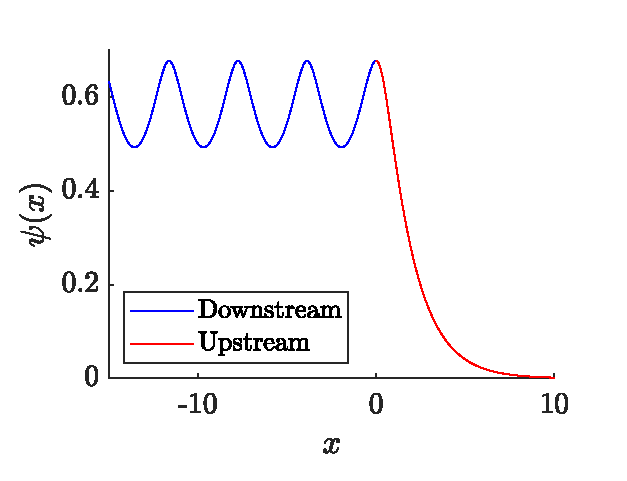
\includegraphics[width=\textwidth]{Sh_M1-300_tau200.eps}
\caption{Down- and upstream}\label{fig:Sh-ex-a}
\end{subfigure}%
\quad
\begin{subfigure}[b]{0.4\textwidth}%[t]{0.5\textwidth}
\centering
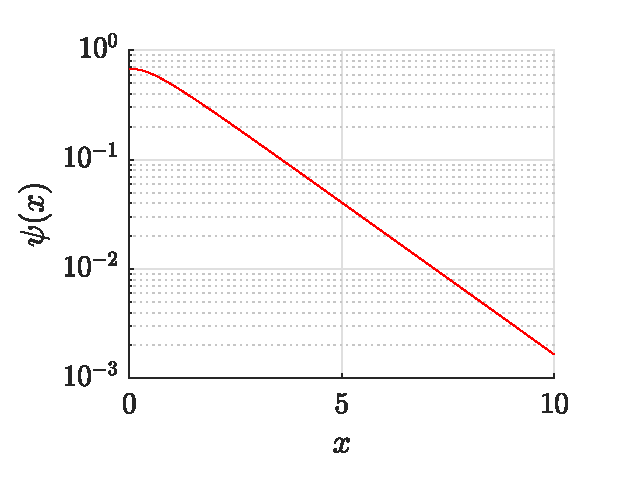
\includegraphics[width=\textwidth]{Sh-US_M1-300_tau200.eps}
\caption{Upstream with log scale}\label{fig:Sh-ex-b}
\end{subfigure}
\caption{Example of the electrostatic potential of a shock (a). In (b)
  the upstream portion of the shock is shown in a log scale, to show
  that $\psi(x)$ decays exponentially for high $x$.
}\label{fig:Sh-ex}
\end{figure}

To export the shock to Gkyl, we need some expression for $\psi(x)$ and
$E(x)$ which can be evaluated at an arbitrary $x$ point. However, sine
the semi-analytical model only produces $\psi$ and $E$ values at
discrete points, we have to create some kind of analytical
approximation.

\subsection{Downstream approximation}
The downstream part of the shock is oscillating with a fixed
wavenumber, as we can see in \figref{fig:Sh-ex-a}. This means that we
can express $\psi(x<0)$ with a Fourier series. Since we further know
that $x=0$ is a maximum of $\psi$, $\dv*{\psi}{x}$ must be $0$ at
$x=0$, meaning that we only need a cosine expansion.

Since the raw data is discrete, it can not be used directly to find
the Fourier coefficients. Instead a cubic spline interpolation is
calculated on all the downstream data points. The coefficients are
calculated using fft on one wavelength, which is densely sampled (1024
points) with the spline.

To be able to find the precise wavelength, $\lambda$, of the
oscillations, the local maxima and minima of $\psi(x)$ are calculated
analytically from the spline interpolation. This is done using the
function \mcode{spline_extrema.m}~[sec.~\ref{sec:spline_extrema}].
Given the wavelength of the oscillation, we can also define a base
frequency $K=2\pi=\lambda$ of the Fourier series.

In the end, the approximate downstream potential becomes
\begin{equation}
\tilde{\psi}(x<0) = \sum_{i=0}^{n_\text{F}} C_{i}\cos(iKx),
\end{equation}
where $n_\text{F}$ is the number of Fourier modes to use in the
approximation. This can also easily be differentiated to give the
approximate electric field and charge density,
\begin{equation}
\begin{aligned}
&\tilde{E}(x<0)=-\dv{\tilde\psi}{x}
=\sum_{i=1}^{n_\text{F}} iKC_{i}\sin(iKx),\\
&\tilde\rho(x<0)=-\dv[2]{\tilde\psi}{x}
=\sum_{i=1}^{n_\text{F}} (iK)^2C_{i}\cos(iKx),\\
\end{aligned}
\end{equation}

\subsection{Upstream approximation}
In the upstream we can use the fact that the potential is
exponentially decaying for large $x$, \figref{fig:Sh-ex-b}, but we
also need to take into account the behavior near the peak.
To do that we fit a rational function $r(x)=p(x)/q(x)$ to
$\log(\psi(x))$. To take the asymptotic behavior into account we can
choose
\begin{equation}\label{eq:pq}
\begin{aligned}
p(x)&= B_2x^n+B_1x^{n-1} + \log(\psi_{\max}) + \sum_{k=2}^{m}A_kx^k\\
q(x)&= x^{n-1}+1,
\end{aligned}
\end{equation}
where $B_2$ and $B_1$ are given by the linear asymptote of
$\log(\psi(x))$. The constant term, $\log(\psi_{\max})$, is there to
get the right value at $x=0$. The fit is then done on the remaining
polynomial coefficients $A_k$, by fitting $p(x)$ to
$q(x)\log(\psi(x))$. Notice that there is no $A_1$, since we 
want $\dv*{r}{x}=0$ at $x=0$.
To determine the values of $B_1$ and $B_2$, a cutoff point,
$x=x_\text{co}$, has to be chosen above which a linear fit is made to
$\log(\psi(x))$. 

Spelled out fully, we get the upstream approximation as
\begin{equation}
\tilde\psi(x>0) = \ee^{r(x)}=\exp(\frac{p(x)}{q(x)})
=\exp(\frac{B_2x^n{+}B_1x^{n-1}{+}\log(\psi_{\max}) +
  \sum_{k=2}^{m}A_kx^k}
{x^{n-1}+1}),
\end{equation}
and the approximate electric field and charge density are
\begin{equation}
\tilde{E}(x>0) = -\dv{\tilde\psi}{x}=r'(x)\ee^{r(x)}
= -r'(x)\tilde\psi(x),
\end{equation}
and
\begin{equation}
\tilde{\rho}(x>0) = \dv{\tilde{E}}{x}
%=\qty[r''(x)+(r'(x))^2]\ee^{r(x)}
=-r''(x)\tilde\psi(x)-r'(x)\tilde{E}(x),
\end{equation}
where ``prime'' denotes derivatives and
\begin{equation}
r'(x)=\dv{r}{x}
=\frac{p'}{q}-\frac{pq'}{q^2}
=r(x)\qty[\frac{p'(x)}{p(x)}-\frac{q'(x)}{q(x)}]
\end{equation}
and
\begin{equation}
r''(x)=\dv[2]{r}{x}
=r(x)\qty[\frac{p''}{p}-\frac{q''}{q}
+2\qty(\frac{q'}{q})^2-2\frac{p'q'}{pq}].
\end{equation}


\subsubsection{Problem with too high degree polynomials}
\label{sec:poly-deg}
There are a couple of free parameters to choose when making an
approximation like this. One of them is the degree, $n$, of the
polynomial to use. The most intuitive idea is that the higher $n$ and
$m$ are the better the fit will be. But there is a very real risk of
over-fitting the polynomials, i.e. introducing artificial variations
between data points. This problem of over-fitting is especially
noticeable in the derivatives. So, since we need to input the electric
field into the initial conditions in Gkyl, we have to be careful to
check that the electric field does not show too many signs of
over-fitting.

The best way to prevent errors due to over-fitting, is to check both
the fit of $\psi(x)$ and $E(x)$. If the fit is bad, then try with a
different $n$. (Usually the best fit is with just keeping $m=n-2$.) It
also need not be that $n$ is too high, sometimes there are some
sweet-spots in the range $n=15{-}25$. Another trick is to try with
ever so slightly different values of $B_{1,2}$, by changing the
asymptotic cutoff point, $x_\text{co}$.





\section{How to use this package (needs updating)}
\begin{center}
\noindent\fbox{
\parbox{14.5cm}{
\textcolor{red}{IMPORTANT NOTE:}
You must have an environment variable \texttt{SHOCKLIB} leading to the
ShockLib directory
(e.g. \texttt{/home/andsunds/SVN/erc/andsunds/Shock-project/ShockLib}),
to run the examples in this package. To
test if you have this environment variable run the command:
\\[.5ex]
\texttt{\$: echo \$SHOCKLIB}
\\[.5ex]
If you do not have it (above command returns empty), run:
\\[.5ex]
\texttt{\$: export SHOCKLIB=<path to Shock library directory>}
\\[.5ex]
This line can also be added to your \texttt{.bashrc} file or
equivalent.
}}
\end{center}

In this section we give a short walk-through of the process of running
a Gkyl simulation of the semi-analytical shocks -- all the way from
choosing the shock parameters to the Gkyl initialization script. 

\subsection{The Matlab part}
The semi-analytical shocks are implemented in Matlab through a shock
class, so all calculations regarding the shock is done through a
\emph{shock object}. This shock object is initialized with the input
parameters:
\begin{itemize}
\item[\texttt{Z} --] ion charge number (may be a vector)
\item[\texttt{m} --] ion mass (may be a vector)
\item[\texttt{n} --] ion initial density (may be a vector)
\item[\texttt{tau} --] electron-to-ion temperature ratio
($T_{\ee}/T_{\ii}$)\footnotemark{}
\item[\texttt{Mach} --] the shock Mach number
\item[\texttt{tol} --] the numerical tolerance wanted
\end{itemize}
The shock initialization also requires an initial guess of
$\phi_{\max}$ and $\phi_{\min}$, \mcode{psimaxmin_in}. The closer
this guess is to the true value, the higher the chances are of
numerical convergence and the faster the shock calculation will run.
\\
To initialize a shock object use e.g.\\
\indent\mcode{Sh0=Shock\_MB(Z,m,n, tau, Mach, psimaxmin_in, tol)};\\
\mcode{Sh0} is now a shock object of the class \mcode{Shock_MB}, and
displaying it should produce an output like:
\vspace{-1em}
\begin{lstlisting}[frame=single]
Shock_MB with properties:

       tol: 1.0000e-09
         Z: 1
         m: 1
         n: 1
      taui: 200
         M: 1.3000
    psimax: 0.6775
    psimin: 0.4929
\end{lstlisting}
Note that \mcode{taui} ($\tau_{\jj}$) is listed here instead of the
input \mcode{tau}. If any of the values listed here are \mcode{NaN},
then the code did not converge, and you need to try some other
\mcode{psimaxmin_in} (or combination of \mcode{Mach}
and \mcode{tau}). 
 
\footnotetext{ This is similar to $\tau_{\jj}$, but without the factor
  $Z_{\jj}$. Also, as of now, different ion temperatures has not been
  implemented.}

\paragraph{Shock classes}
There are currently two shock classes supported in the
\mcode{Shock_pkg_new} package:
\begin{itemize}
\item \mcode{Shock_MB(Z,m,n, tau, Mach, psimaxmin_in, tol)}\\
the simplest type of shock, with Maxwell-Boltzmann distributed
electrons. 
\item \mcode{Shock_col(Z,m,n, tau, Mach, t0, nustar, psimaxmin_in, tol)}\\
which is our collisional shock model. 
\end{itemize}
Note that the different classes require different input parameters.

There are also classes for electron trapping under development in this
new package. (There already exists electron trapping classes in the
original shock package, \mcode{Shock_pkg}, but not in this one with
the new normalization.)


\subsubsection{Calculating the electrostatic potential}
Using this shock object, the electrostatic potential is then easily
calculated with the built-in function\\
\indent\mcode{[X,psi]=Sh0.find_psi(xmin,xmax)},\\
which operates on the shock object \mcode{Sh0}, and calculates its
electrostatic potential in the range \mcode{xmin} to \mcode{xmax}.

When calculating the electrostatic potential, we cannot use a too
large range in $x$. This is because at large positive $x$, where
$\psi$ is very close to zero, numerical errors can affect the result
and become unstable. An example of this is shown in
\figref{fig:too-large-range}. To avoid these types of errors, we have
to manually check that the potential looks okay. There is also a
tendency to get complex numerical values when this happens.

If we want to, we can also get the electric field and charge density
at the same time by running:\\
\indent\mcode{[X,psi,E,rho]=Sh0.find_psi(xmin,xmax)}\\
The electric field and charge density are useful, but not required, if
we also want to find the approximation later on.

\begin{figure}
\centering
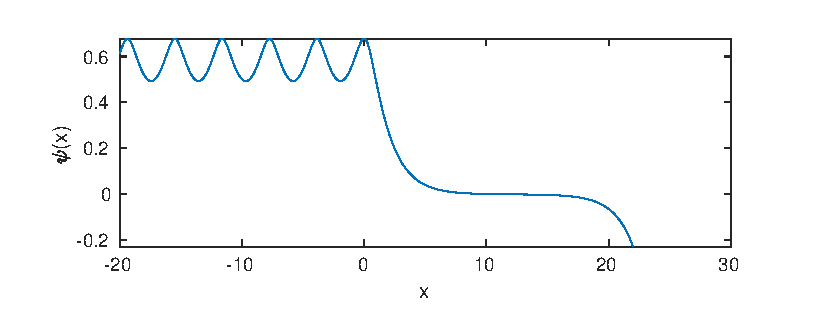
\includegraphics{Sh_M1-300_tau200_too-large-range.eps}
\caption{Erroneous potential, $\psi$, due to numerical error which
  manifest at large positive $x$ values.}
\label{fig:too-large-range}
\end{figure}

\subsubsection{Finding the exportable approximation}
Now that we have found $\psi$, $E$, and $\rho$, we can use them to find
the approximations described in Section~\ref{sec:approx}. To do that
we have the function\\
\indent\mcode{[Cm, K, Cp] = find_approx(X,psi,E,rho,N_sample,exp_threshold,poly_deg)}\\
which takes in the discrete \mcode{X}, \mcode{psi}, \mcode{E}, and
\mcode{rho} and calculates the approximation coefficients in the
negative $x$ range, \mcode{Cm}, as well as for positive $x$,
\mcode{Cp}. In the negative $x$ range, \mcode{K} is the base frequency
of the cosine series. The positive approximation coefficients,
\mcode{Cp}, are just all polynomial coefficients of $p(x)$ arranged in
increasing powers.

For a list of the other input arguments to this function, see
Section~\ref{sec:find_approx}. 

It is possible to run \mcode{find_approx} without giving \mcode{E} and
\mcode{rho}. This will work in most cases, but it will be harder to
find a good fit. 


As was mentioned in Section~\ref{sec:poly-deg}, there are some manual
work required to get a good fit. It is therefore recommended to also
use\\
\indent\mcode{[psi,E,rho] = get_approx(X,Cm,K,nf, Cp)}\\
to check that the approximation functions are satisfactory (also in
$E$), and if needed experiment with \mcode{poly_deg} and
\mcode{exp_threshold}. This function takes the approximation
coefficients, \mcode{Cm} and \mcode{Cp}, and returns the approximate
values of $\psi$, $E$, and $\rho$ at the points specified in
\mcode{X}. The argument \mcode{nf} is the number of frequencies
(cosine terms) to use for the DS approximation.

\paragraph{Export protocol}
When we have found a satisfying approximation, we have to save the
coefficients to file. This is done in a function\\
\indent\mcode{[save_data] = save_coefs(save_path,Cm,K,Cp)}\\
which saves the coefficients in a tsv-file with the correct
format~[sec.~\ref{sec:save_coefs}]. The \mcode{save_path} is a string
with the path and fime name, to which the coefficients will be
saved. Also, \mcode{Cm} should only contain the \mcode{nf} number of
coefficients as you want to save.

When saving, you will be prompted if you want to save the coefficients
to the path provided or not.


\subsubsection{Other things to do with the shock classes}
We do, of course, not all the time want to calculate $\psi(x)$. This
is a bit outside the scope of these instruction notes but some other
functions in the \mcode{Shock_pkg_new} package are
\begin{itemize}
\item \mcode{[Sh_cell] = t_sweep(pre_calc_Shock,i0,N_steps,t0,output_file)}\\
A function to be used with \mcode{Shock_col} objects, for sweeping
through time to see how the collisions evolve the shock. The output is
a cell list filled with shock objects for each time step.
\item \mcode{[Sh_cell] = tau_sweep(pre_calc_Shock,i0,N_steps,tau0,dtau)}\\
A function for sweeping through different \mcode{tau} values, and
recording how the shock behavior changes. 
\item \mcode{[Sh_cell] = Mach_sweep(Sh_handle,pre_calc_Shock,i0,N_steps,M0,dM)}\\
A function for sweeping through different \mcode{Mach} values.
\item \mcode{[Sh_cell] = M_tau_sweep(pre_calc_Shock,iT0,TT,iM0,M0,dM,NM)}\\
This function does a 2D scan for different \mcode{Mach} and
\mcode{tau} values. For each \mcode{tau} value, the function sweeps
through the \mcode{Mach} range.
\end{itemize}
In each of these scanning/sweeping functions, each new step is
initialized with the \mcode{psimax} and \mcode{psimin} of the previous
step. In all but the time scan, the function tries a step and if it
doesn't work, takes a half step back and tries again. By doing this
the ends of the each corresponding range can be studied with less
manual supervision.

\subsection{The Gkyl part}
Once the approximation coefficients have been saved in the proper
format, we can head over to Gkyl to import the shock. With the help of
the \texttt{shApprox} package [sec.~\ref{sec:shApprox}], this is done
quite easily. First, we need to add it to the package path, which is
done with the line\\
\indent\texttt{package.path = package.path..";"..<path to shApprox.lua>}\\
Then we also need to import the package:\\
\indent\texttt{local Approx = require "shApprox"}\\
In our example the path to the package can be written as\\
\indent\texttt{os.getenv("SHOCKLIB").."/luaLib/?.lua"}\\
This adds any file in the path
\texttt{\$SHOCKLIB/luaLib/}, ending with
\texttt{.lua}, to the list of packages. (The operator \texttt{..} is
string concatenation in Lua.)
Another central part of the \texttt{shApprox} package is the
coefficient file, whose filename is passed around a lot. It is
therefore a good idea to also have a variable\\
\indent\texttt{local filename = "<path to coef file>"}\\
with the path and file name of the coefficient file.

The next step is to set all the parameters for the simulation. Please
see the example input file for a more details of the way of doing
this. In some more general terms, one way of setting up the input
parameters is to use some units when defining, for instance, the masses
of the species, e.g. \texttt{me\_hat=1} and \texttt{mi\_hat=1836.153},
and then use them in the normalized quantities as described in
Section~\ref{sec:norm}. We must also keep the comments in
Section~\ref{sec:zeta}, about $\zeta$ and how Gkyl wants mass and
charge separately, in mind.

When initializing the species, we have to provide the distribution
functions for each species and fields. This is also easily done
through the \texttt{shApprox} package which has the functions\\
\indent\texttt{fi(x,v, ni0,taui, zetai, M, filename, dv)},\\
\indent\texttt{fe\_MB(x,v,ne1,zetae,M,filename)}, and\\
\indent\texttt{Ex(x, filename)},\\
which calculates precisely the distribution functions and fields that
we want. The input argument \texttt{dv} is the simulation grid size in
velocity, and is used to create a more smooth transition to the empty
regions of phase-space. Also note that the electron distribution
function takes \texttt{ne1}, i.e. \eqref{eq:ne1}, as its input
argument.  

For other inquiries regarding the Gkyl part, the reader is referred to
the example script and the Gkyl manual,
\url{http://gkyl.readthedocs.io/en/latest/}.


\section{Code documentation (needs updating)}
This package consists of libraries with scripts for Matlab and
Lua. The Matlab library concerns the semi-analytical shocks, and
fining their approximations. The Lua library is just a single package
that takes the approximation coefficients given by the Matlab scripts,
and gives the wanted function values in Lua.

\subsection{mLib/}
The Matlab library has four functions, \mcode{find_approx},
\mcode{get_approx}, \mcode{save_coefs}, and
\mcode{spline_extrema}. All exept \mcode{spline_extrema} are directly
used by the user.  

\subsubsection{\texttt{find\_approx.m}}
\label{sec:find_approx}
\mcode{[Cm, K, Cp] = find\_approx(X,psi,E,rho,N\_sample,exp\_threshold,poly\_deg)}
\\[1ex]
This function calculates the approximation coefficients, \mcode{Cm},
\mcode{K}, and \mcode{Cp}, according to the approximation schemes
described in Section~\ref{sec:approx}.

This function takes in the true values of \mcode{psi}, \mcode{E}, and
\mcode{rho}, this is the recommended way of running this
function. However, this function can be run with only \mcode{psi} as
input, although the US fit will not be as good. The other input
arguments are
\begin{itemize}
\item \mcode{N_sample} is the number of sample points to be used in the FFT
of the DS oscillation.
\item \mcode{exp_threshold} is the cut-off point, $x_\text{co}$, above which
$\psi$ is said to be decaying exponentially.
\item \mcode{poly_deg} is the degree, $n$, of the numerator polynomial,
$p(x)$; \mcode{poly_deg} may also be a two component vector, in that
case, the second element is the degree, $m$, of the fitted part of
$p(x)$ [see \eqref{eq:pq}].
\end{itemize}


\paragraph{Downstream approximation}
Since the DS oscillation is periodic, we should be able to fit a Fourier
series to it. We also know that $\eval{\dv*{\psi}{x}}_{x=0}=0$, which
leaves us with only the cosine terms (i.e. the real part of complex
F-coefficients). However, as the data points are unevenly spaced, and
not aligned with the exact period of the oscillation, we first need to
create a cubic spline interpolation to get the exact period. Then we
use the dedicated function, \mcode{spline_extrema}, that finds the
analytical min/max points of the cubic spline of the DS
oscillations. With the location of the extremum points, we can
determine the wavelength, $\lambda$, of the first (closest to $x=0$)
oscillation. (We want to use the first oscillation, since that has the
least numerical errors, from the ODE solver, in it.)

Then we create a densely sampled version of $\psi(x)$ in this first
wavelength, with \mcode{N_sample} sampling points, using the spline
interpolation. We can then find the F-coefficients with FFT. Finally
we convert the complex Fourier transform into a cosine transformation
by only choosing the real part of the complex coefficients, and also
doubling the non-zero frequency terms. The FFT does give some
imaginary parts to the coefficients, but they are a couple of orders
of magnitude smaller that the real parts, so it is indeed safe to
discard the sine terms of the Fourier series.


\paragraph{Upstream approximation}
We want to fit the rational function, $r(x)=p(x)/q(x)$, where $p$ and
$q$ are given by \eqref{eq:pq}, to $\log(\psi(x))$. First, $B_1$ and
$B_2$ are chosen by finding a linear fit to $\log(\psi(x))$ for
$x>$\,\mcode{exp_threshold}. Then the lower order coefficients, $A_k$,
are fitted using a least square fit on all the data points.

If \mcode{E} and \mcode{rho} are given at the input, the first two
coefficients, $A_2$ and $A_3$, are set to be the corresponding Taylor
coefficients of
\begin{equation}
q(x)\log(\psi(x)) = (x^{n-1}+1)\,\log(\psi(x)),
\end{equation}
which are
\begin{equation}
\begin{aligned}
&A_2 = \frac{1}{2\psi_{\max}}\eval{\dv[2]{\psi}{x}}_{x=0}
= \frac{\rho(x=0)}{2\psi_{\max}}\\
&A_3 = \frac{1}{6\psi_{\max}}\eval{\dv[3]{\psi}{x}}_{x=0}
= -\frac{1}{6\psi_{\max}}\eval{\dv{\rho}{x}}_{x=0}.
\end{aligned}
\end{equation}
The rest of the coefficients are then fitted with zero as the initial
guess for all of them. If, on the other hand, \mcode{E} and
\mcode{rho} are not given at the input, then also $A_2$ and $A_3$ are
subject to fitting. 


\subsubsection{\texttt{get\_approx.m}}
\indent\mcode{[psi,E,rho] = get_approx(X,Cm,K,nf,Cp)}\\
This is a function that gets the value of the
approximation~[sec.~\ref{sec:approx}] in the points \mcode{X}, given
the approximation coefficients \mcode{Cm} and \mcode{Cp}. The other
arguments, \mcode{K}, is the frequency of the downstream oscillations,
and \mcode{nf} is the number or Fourier modes to use in the
approximation. (Usually Cm is 1024 elements long, and we only need the
first $\order{10}$ modes to get an accurate representation.) 
The main use of this function is to display the result of 
\mcode{find_approx} to manually inspect how good the fit is.

Thi function can also calculate the approximate electric field,
\mcode{E}, and the charge density, \mcode{rho}. This is done
analytically, with the analytical derivatives of the approximation
functions. 


\subsubsection{\texttt{save\_coefs.m}}
\label{sec:save_coefs}
\indent\mcode{[save_data] = save_coefs(save_path,Cm,K,Cp)}\\
Arranges the approximation coefficients into a matrix,
\mcode{save_data}, and propts you if you want to save it to the path
provided in \mcode{save_path}.
The format in which the coefficients have to saved are as follows:
\vspace{-1.5em}
\begin{lstlisting}
 K     Cp_0
Cm_0   Cp_1
Cm_1   Cp_2
 |      |
 0     Cp_n
\end{lstlisting}
That is, two columns, with the first one starting with the base
frequency of the DS oscillations, \mcode{K}, and then followed by the
coefficients of the cosine series, \mcode{Cm}. The second column
instead consists of all the polynomial coefficients of $p(x)$.

The downstream coefficient vector, \mcode{Cm}, should only contain the
Fourier coefficients that you want to save. So the first column ends
with zeros, since in general not as many cosine coefficients are
needed as polynomial coefficients. The first column may be as long as,
\emph{but not longer than}, the second column in terms of values
given. I.e. \textbf{the second column may not end with zeros.} This is
because the Lua package has no way of knowing the degree, $n$, of the
polynomial, $p(x)$, other than looking at the length of the second column.



\subsubsection{\texttt{spline\_extrema.m}}\label{sec:spline_extrema}
This is a function that finds all the extrema of a spline object by
analytically calculating the roots of the derivative of each spline:\\
\indent\mcode{[x0,y0] = spline\_extrema(pp\_spline)}\\
\mcode{x0} and \mcode{y0} are the x and y coordinates of the extremum
points, and \mcode{pp\_spline} is a Matlab spline pp-object.

To find a local extremum of a cubic spline interpolation, we use the
fact that the interpolations consists of multiple cubic polynomials of
the form 
\begin{equation}
S_n(x) = a_n(x-x_{n})^3+b_n(x-x_n)^2+c_n(x-x_n)+d_n
\qfor x_n\le x<x_{n+1}.
\end{equation}
The roots of the derivatives are simply given by the quadratic formula
\begin{equation}
x^{\pm}_n-x_n=\frac{-b_n\pm\sqrt{b_n^2-3a_nc_n}}{3a_n}.
\end{equation}
We call these the pseudo roots, since not all of them represent actual
extremum points of the spline interpolation. The proper roots of the
spline derivatives are the ones that fall inside the interval of their
respective polynomial, $x_n\le x_n^\pm<x_{n+1}$.  



\subsection{luaLib/}
The Lua library only contains one single file, \texttt{shApprox.lua},
which is a package of the different lua functions we would want to use
in Gkyl.

\subsubsection{\texttt{shApprox.lua}}
\label{sec:shApprox}
This script file contains several different function which can be used
by importing this file as a package.

All functions in the user interface takes in a \mcode{filename}
argument, which is the path and name of the file containing the
approximation coefficients. This file must be formatted
correctly~[sec.~\ref{sec:save_coefs}].

All the functions that take an input \mcode{x}, have the convention
that the boundary between up- and downstream, is at \mcode{x = 0}.

\paragraph{\texttt{lambda(filename)}}\mbox{}\\
This function returns the wavelength of the DS oscillations, by
simply using the frequency that is given in \mcode{filename}.

\paragraph{\texttt{psi(x, filename)}}\mbox{}\\
Calculates the approximate electrostatic
potential~[sec.~\ref{sec:approx}] at the point \mcode{x}, given the
approximation coefficients in the file \mcode{filename}. 

\paragraph{\texttt{psimax(filename)}}\mbox{}\\
Calculates the maximum value of the electrostatic potential, given the
coefficients in \mcode{filename}. Gives the same result as
\mcode{psi(0,filename)}. 

\paragraph{\texttt{Ex(x, filename)}}\mbox{}\\
Calculates the approximate electric field analytically at the point
\mcode{x}, given the approximation coefficients in the file
\mcode{filename}. 

\paragraph{\texttt{fi(x,v,ni0,taui,zetai,M, filename, dv)}}\mbox{}\\
Calculates the ion distribution function \eqref{eq:fj} at the
phase-space point \mcode{(x,v)}.

This function does also take into account the ion reflection, meaning
that the distribution function gets cut off above
$v_0=\sqrt{2\zeta_{\jj}(\psi-\psi_{\max})}$ in the upstream
($-v_0$ in the downstream). However, to prevent large errors due to
the velocity discretization in Gkyl, the cut-off is made soft by
having a Gaussian decay, \mcode{math.exp(-10*(v-USDS*v0)^2/dv^2)}. The
Gaussian starts at the cut-off point, \mcode{v-USDS*v0}, where
\mcode{USDS = 1} (\mcode{-1}) in the upstream (downstream), and where
\mcode{dv} is the discretization step size.

\paragraph{\texttt{ni1(ni0,taui,zetai,M, filename)}}\mbox{}\\
Calcualtes the far-upstream ion density \eqref{eq:nj1} by
numerically integrating the ion-distribution, \eqref{eq:fj}, with
$\psi=0$ from $-\infty$ to $v_0=\sqrt{2\zeta_{\jj}\psi_{\max}}$.

\paragraph{\texttt{fe\_MB(x,v,ne1,zetae,M, filename)}}\mbox{}\\
Calcualtes the Maxwell-Boltzmann electron distribution function
\eqref{eq:fe}. Note that \mcode{zetae} is negative since $Z_{\ee}=-1$,
and hence
\begin{equation}
\zeta_\ee=\frac{Z_{\ee}/\hat{m}_{\ee}}{\hcs^2/\hat{T}_{\ee}}
=-\frac{\hat{T}_{\ee}}{\hat{m}_{\ee}\hcs^2}\sim-2000<0.
\end{equation}





%%%%%%%%%%%%%%%%%%%%%%%%%% The bibliography %%%%%%%%%%%%%%%%%%%%%%%%%%
%\newpage
%% This bibliography uses BibTeX
\bibliographystyle{ieeetr}
\bibliography{references}%requires a file named 'references.bib'
%% Citations are as usual: \cite{example_article}

%%%%%%%%%%%%%%%%%%%%%%%%%%%%%%%%%%%%%%%%%%%%%%%%%%%%%%%%%%%%%%%%%%%%%%
\end{document}%% ^ ^ ^ ^ ^ ^ ^ ^ ^ ^ ^ ^ ^ ^ ^ ^ ^ ^ ^ ^ ^ ^ ^ ^ ^ ^ ^
%%%%%%%%%%%%%%%%%%%%%%%%%%%%%%%%%%%%%%%%%%%%%%%%%%%%%%%%%%%%%%%%%%%%%%



%%% Local Variables:
%%% mode: latex
%%% TeX-master: t
%%% End:

%  LocalWords:  Maxwellian MATLAB Gkyl mLib luaLib shApprox lua fft
%  LocalWords:  extremum extrema psimaxmin NaN nustar tol taui psimax
%  LocalWords:  psimin xmin xmax DS Cp USDS
